\documentclass[utf8, diplomski]{fer}
\usepackage{booktabs}
\usepackage{longtable}
\usepackage{ltablex}
\usepackage{pdfpages}
\usepackage{hyperref}
\usepackage{mathtools}
\usepackage{listings}
\usepackage{subfig}
\setcitestyle{numbers,square,super}
\usepackage[export]{adjustbox}
\usepackage{float}


\begin{document}

\thesisnumber{2231}

\title{Obrana dubokih konvolucijskih modela od neprijateljskih primjera}

\author{Matej Dobrovodski}

\maketitle

\iffalse \includepdf[pages=-]{img/content/izvornik.pdf} \fi

\tableofcontents

\chapter{Uvod}
\section{Raspoznavanje objekata}
Raspoznavanje objekata jedan je od ključnih problema područja računalnog vida. Pri rješavanju problema raspoznavanja objekata se na ulaz nekog sustava dovede slika nekog objekta, a na izlazu se očekuje ispravna klasifikacija u neki od predodređenih razreda. Čovjeku ovaj zadatak ne predstavlja veliki problem, no još uvijek ne postoji zadovoljavajuće rješenje problema koje bi vrijedilo za opći slučaj. Trenutno najbolja takva rješenja temelje se na konvolucijskim neuronskim mrežama. \par
Razvoj konvolucijskih mreža počeo je osamdesetih godina prošlog stoljeća. Počelo je razvojem \textit{neocognitron}[citat?]-a--neuronske mreže inspirirane biološkim stanicama vidne kore mozga. Krajem devedesetih godina se pojavljuje konvolucijska neuronska mreža LeNet5. LeNet5 mreža je vrlo uspješno raspoznavala rukom pisane znamenke te je ova mreža bila početna točka za daljnja istraživanja drugih neuronskih mreža. [citati] \par
\textit{ImageNet}[citat] projekt je velika baza podataka predviđena za istraživanje područja raspoznavanja objekata. S više od $14$ milijuna slika podijeljenih u $20000$ kategorija, \textit{ImageNet} skup je daleko najveći slobodno dostupni skup. Počevši od 2010.[?] godine, \textit{ImageNet} projekt organizira godišnje natjecanje, \textit{ImageNet Large Scale Visual Recognition Challenge} (ILSVRC). Veliki skok u točnosti pri raspoznavanju dogodio se 2012. godine kada je konvolucijska neuronska mreža \textit{AlexNet}[citat] postigla top-5 pogrešku od samo $15.3\%$, što je bilo $10.8\%$ manje od sljedeće mreže. To je postignuto korištenjem grafičkih procesora pri treniranju, što je potaknulo svojevrsnu revoluciju u području dubokog učenja. \par
Do 2017. godine, većina timova u natjecanju je imala top-5 točnost veću od $95\%$. Danas se u raznim bibliotekama mogu naći unaprijed istrenirane mreže koje postižu vrlo dobre rezultate, te će se one spominjati i koristiti u nastavku rada. Neke od njih su \textit{ResNet}[citat], \textit{Xception}[citat] i \textit{VGG}[citat]. Sve spomenute mreže postižu vrlo zadovoljavajuće točnosti pri ispitivanju (top-5 točnosti iznad $90\%$) i čini se da mogu dobro generalizirati. No u nastavku rada će biti pokazan oblik napada na konvolucijske mreže koji dovodi u pitanje činjenicu da današnje konvolucijske mreže dobro generaliziraju.
\section{Neprijateljski primjeri}
Krajem $2013.$ godine pojavljuje se prvi izravni "napad" na duboke neuronske mreže\citep{Szegedy2014IntriguingPO}, gdje je jedna od meta bila prethodno spomenuta uspješna mreža \textit{AlexNet}. Polazna pretpostavka je da duboki modeli, usprkos tome što dobro generaliziraju, imaju ugrađene svojevrsne \textit{slijepe pjege} koje se isplati istražiti.
\par
Vrijedi da za neki ispravno klasificirani ulaz $x$ postoji područje u blizini ulaza, $x + r$, gdje je $||r|| < \epsilon$ za neki dovoljno mali radijus $\epsilon > 0$. Uobičajeno je da modeli ulazne vrijednosti iz tog područja također ispravno klasificiraju, kao i $x$, te u općem slučaju vrijedi da neprimjetne perturbacije iz tog $\epsilon$ područja (npr. nasumični šum slabog intenziteta) ne mijenjaju izlaz modela. Rješavanjem optimizacijskog problema pri kojem se minimizira perturbacija $r$ koja izaziva pogrešnu klasifikaciju dolazzi se do takozvanih neprijateljskih (ili suparničkih) primjera (eng. \textit{adversarial example}). Ono što je iznenađujuće i što je potaklo daljnje istraživanje je to što je zapravo vrlo lako za pronaći neprijateljske primjere na \textit{state of the art} modelima kod kojih je perturbacija $r$ praktički potpuno neprimjetna i gdje nije očito zašto mreže neispravno klasificiraju takve ulaze. U nastavku rada je dan pregled nekoliko metoda generiranja neprijateljskih primjera: neke metode su prikazane zbog njihove povijesne važnosti i utjecaja na daljni razvoj metoda, dok su neke metode iznimno snažne i mjerilo za uspješnost obrane od suparničkih napada. Uz napade su pokazane i obrane, s naglaskom na njihovu (ne)uspješnost pri odupiranju od suparničkih napada, probleme koji su im zajednički te potencijalnu budućnost razvoja uspješnijih obrana.

\chapter{Programska potpora}
\section{Odabir biblioteke za duboko učenje}
tensorflow\citep{abadi2016tensorflow} keras\citep{chollet2015keras}
\section{Biblioteke za neprijateljske primjere}
foolbox\citep{rauber2017foolbox} cleverhans\citep{papernot2018cleverhans} art\citep{art2018}
\section{Skupovi podataka}
imagenet, cifar10, personal
\section{Konvolucijski modeli}
resnet, etc, onaj mali model


\chapter{Neprijateljski primjeri I}
\section{Model prijetnje}
Osnovni termini, lažno pozitivni/negativni(*) primjeri, white/black box, targeted/nontargeted, one-time/iterative \citep{Yuan2019AdversarialEA}
\section{Pojava prvih neprijateljskih primjera}
intriguing properties\citep{Szegedy2014IntriguingPO}
\section{Brza metoda temeljena na gradijentima}
fg(s)m\citep{Goodfellow2015ExplainingAH}
\section{DeepFool} df\citep{MoosaviDezfooli2016DeepFoolAS}


\chapter{Obrana dubokih konvolucijskih modela}
opisati vrste obrane \\

\chapter{Neprijateljski primjeri II}
\section{Neučinkovitost obrana} ...
\section{PGD} pgd\citep{Madry2017TowardsDL}
\section{Napadi \textit{Carlini and Wagner}} candw\citep{Carlini2017TowardsET}
\section{Napad temeljen na odluci} boundary\citep{Brendel2017DecisionBasedAA}

\chapter{Budućnost obrana od neprijateljskih napada}
\section{PGD adversarial training}
\section{Preduvjeti uspješnih obrana}
\section{Dokazivost obrane od neprijateljskih napada}
\section{Budući rad}

\chapter{Zaključak}
Konvolucijske neuronske mreže su se pokazale iznimno uspješnima pri rješavanju problema klasifikacije objekata. Međutim, pojava neprijateljskih primjera postavlja 


\bibliography{literatura}
\bibliographystyle{fer}

\chapter{Dodatak}
\section{Osobni skup slika}
U \ref{ref_personal_image_table} je $16$ slika i labela koje su u radu korištene za generiranje suparničkih primjera za modele trenirane na \textit{ImageNet} skupu podataka. Sve slike su odabrane tako da spadaju unutar $1000$ razreda za koje su modeli predviđeni, dakle slike bi trebale biti ispravno klasficirane. Također, sve slike su unaprijed izrezane u oblik kvadrata kako ne bi došlo do degradacije kvalitete pri smanjenju rezolucije na $224\times224$. Zahvaljujem se Sarah James na dopuštenju za korištenje slika u radu.

\begin{figure}
    \centering
    % images 1-4
    \subfloat[\textit{African grey} (87)]{
        \label{ref_pi1}
        \includegraphics[width=0.25\textwidth]{img/personal_images/african_grey.jpg}
    }
    \subfloat[\textit{Backpack} (414)]{
        \label{ref_pi2}
        \includegraphics[width=0.25\textwidth]{img/personal_images/backpack.jpg}
    }
    \subfloat[\textit{Dragonfly} (319)]{
        \label{ref_pi3}
        \includegraphics[width=0.25\textwidth]{img/personal_images/dragonfly.jpg}
    }
    \subfloat[\textit{Bald eagle} (22)]{
        \label{ref_pi4}
        \includegraphics[width=0.25\textwidth]{img/personal_images/eagle.jpg}
    }
    \newline
    % images 5-8
    \subfloat[\textit{Grocery store} (582)]{
        \label{ref_pi5}
        \includegraphics[width=0.25\textwidth]{img/personal_images/food_market.jpg}
    }
    \subfloat[\textit{Gorilla} (366)]{
        \label{ref_pi6}
        \includegraphics[width=0.25\textwidth]{img/personal_images/gorilla.jpg}
    }
    \subfloat[\textit{Guinea pig} (338)]{
        \label{ref_pi7}
        \includegraphics[width=0.25\textwidth]{img/personal_images/guinea_pig.jpg}
    }
    \subfloat[\textit{Jack-o'-lantern} (607)]{
        \label{ref_pi8}
        \includegraphics[width=0.25\textwidth]{img/personal_images/jackolantern.jpg}
    }
    \newline
    % images 9-12
    \subfloat[\textit{Jigsaw puzzle} (611)]{
        \label{ref_pi9}
        \includegraphics[width=0.25\textwidth]{img/personal_images/jigsaw2.jpg}
    }
    \subfloat[\textit{Keypad} (508)]{
        \label{ref_pi10}
        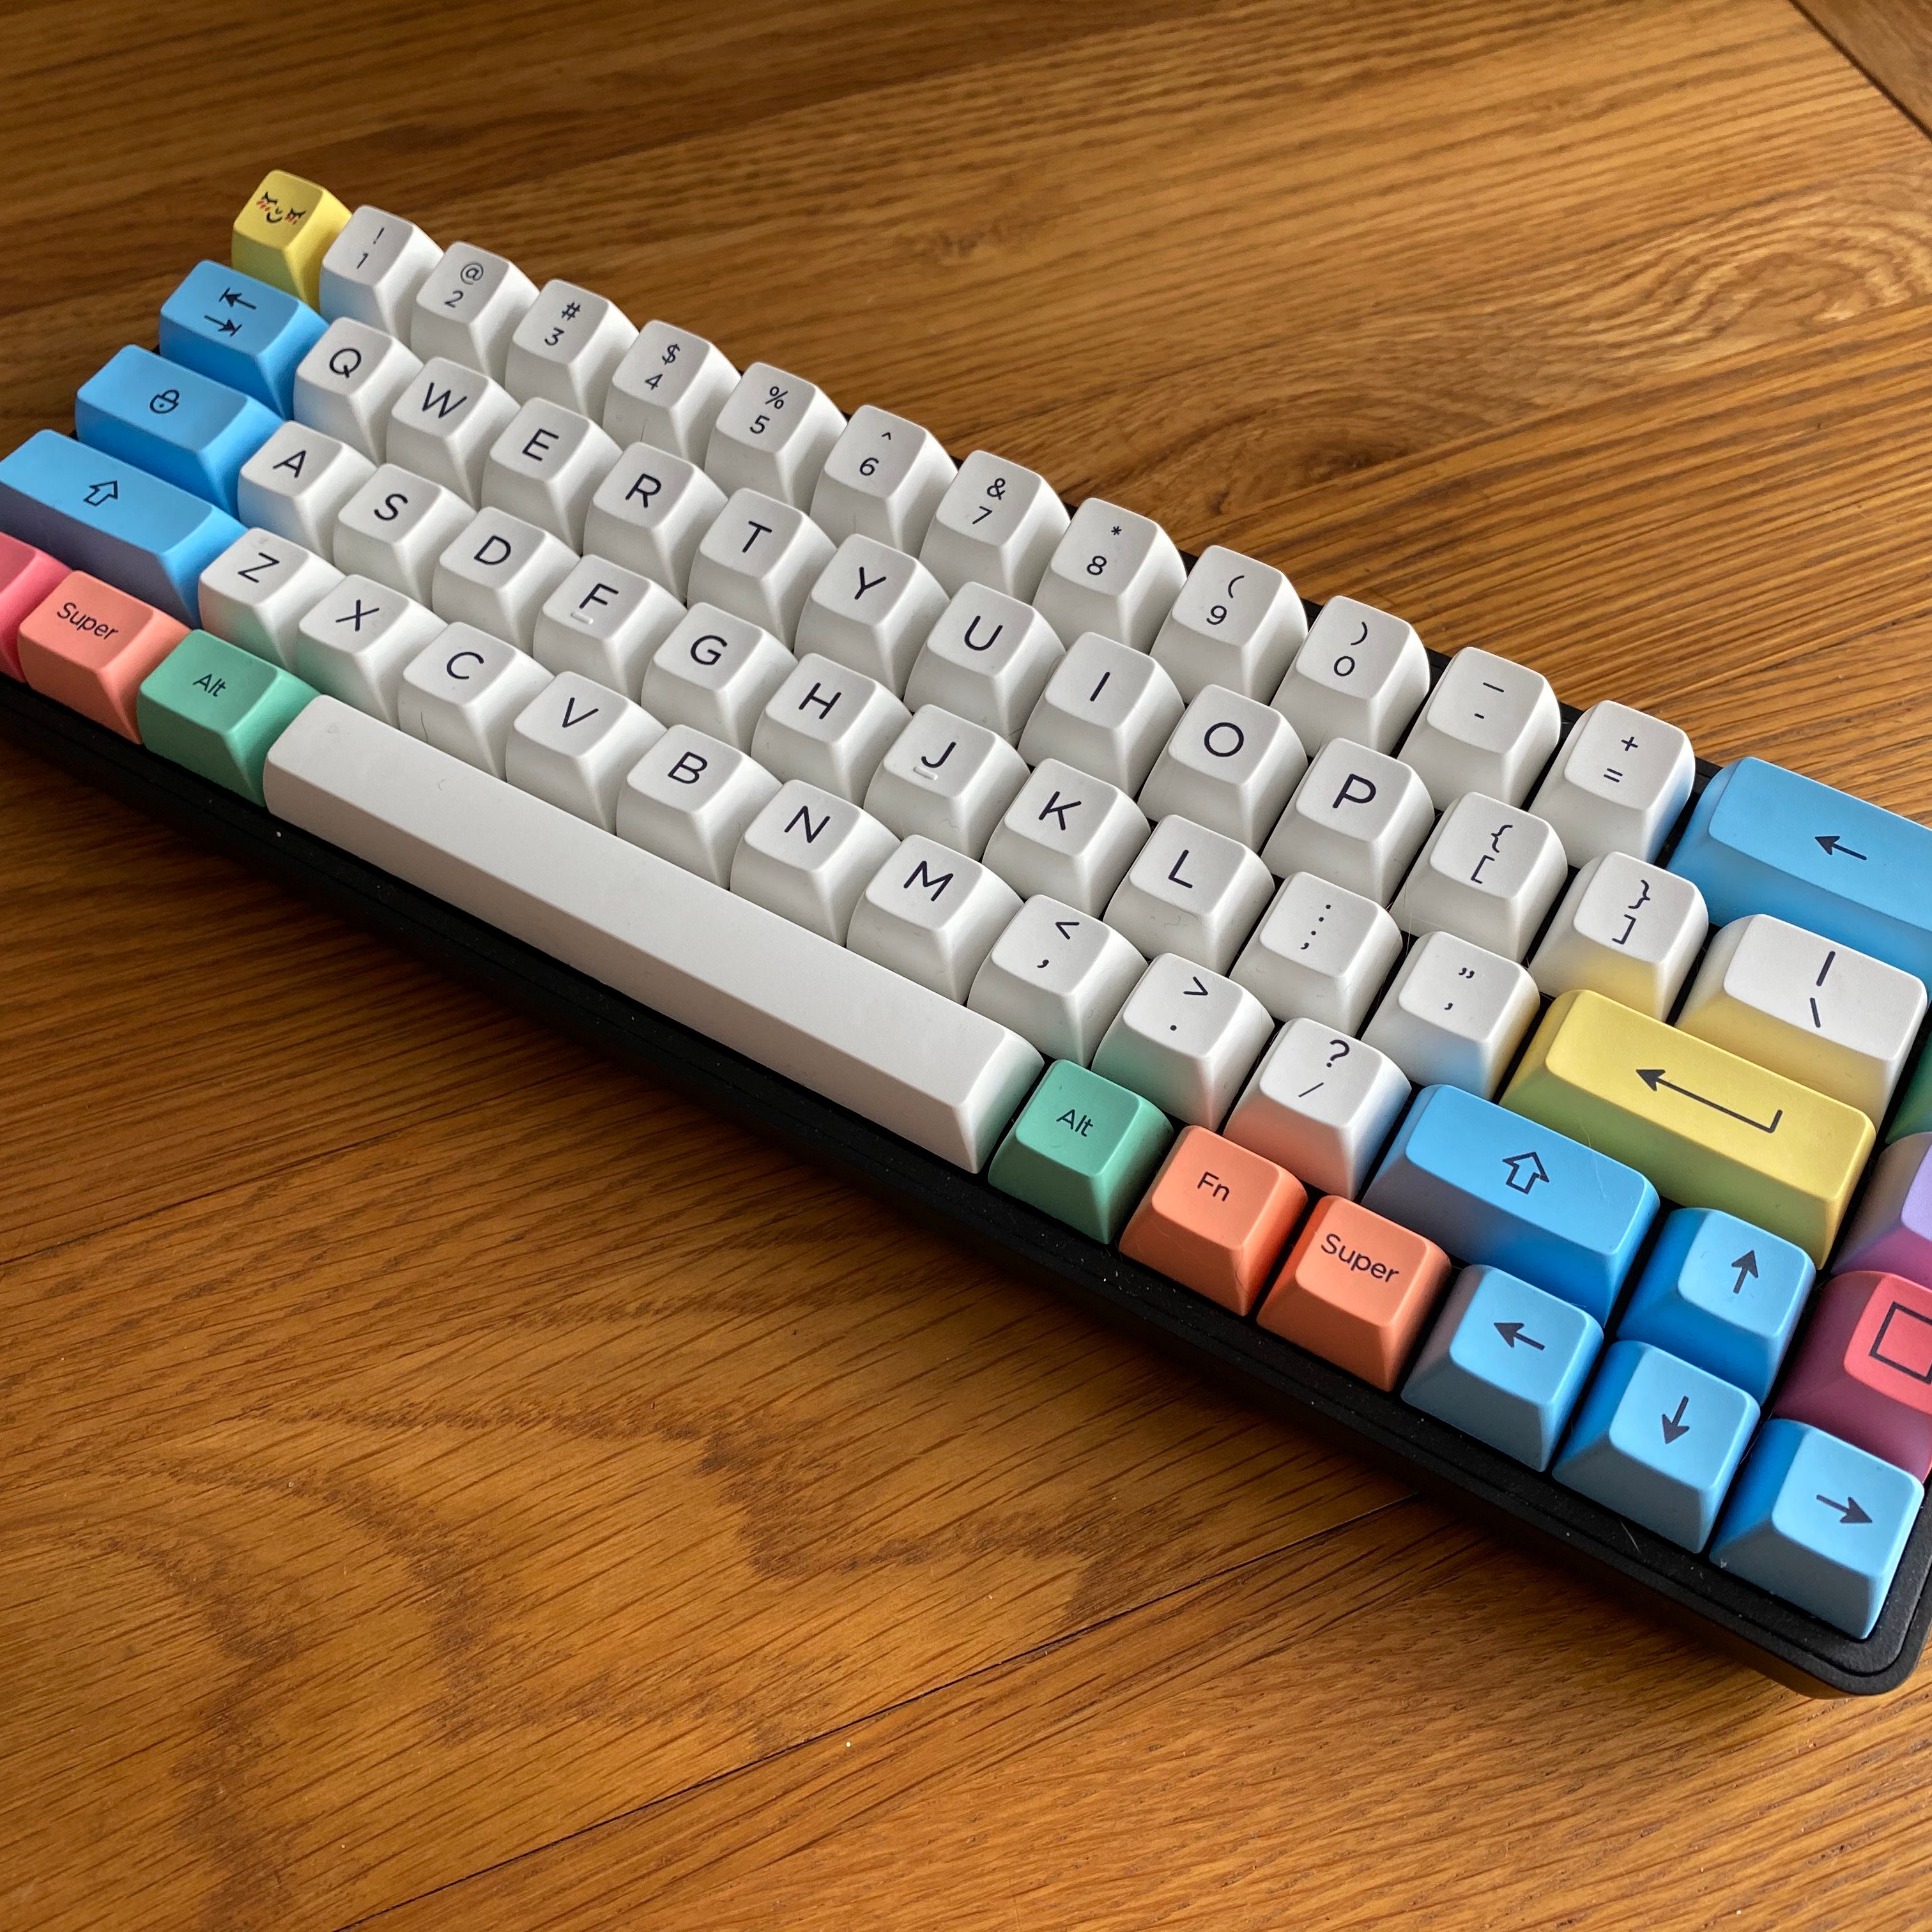
\includegraphics[width=0.25\textwidth]{img/personal_images/keyboard.jpg}
    }
    \subfloat[\textit{Llama} (355)]{
        \label{ref_pi11}
        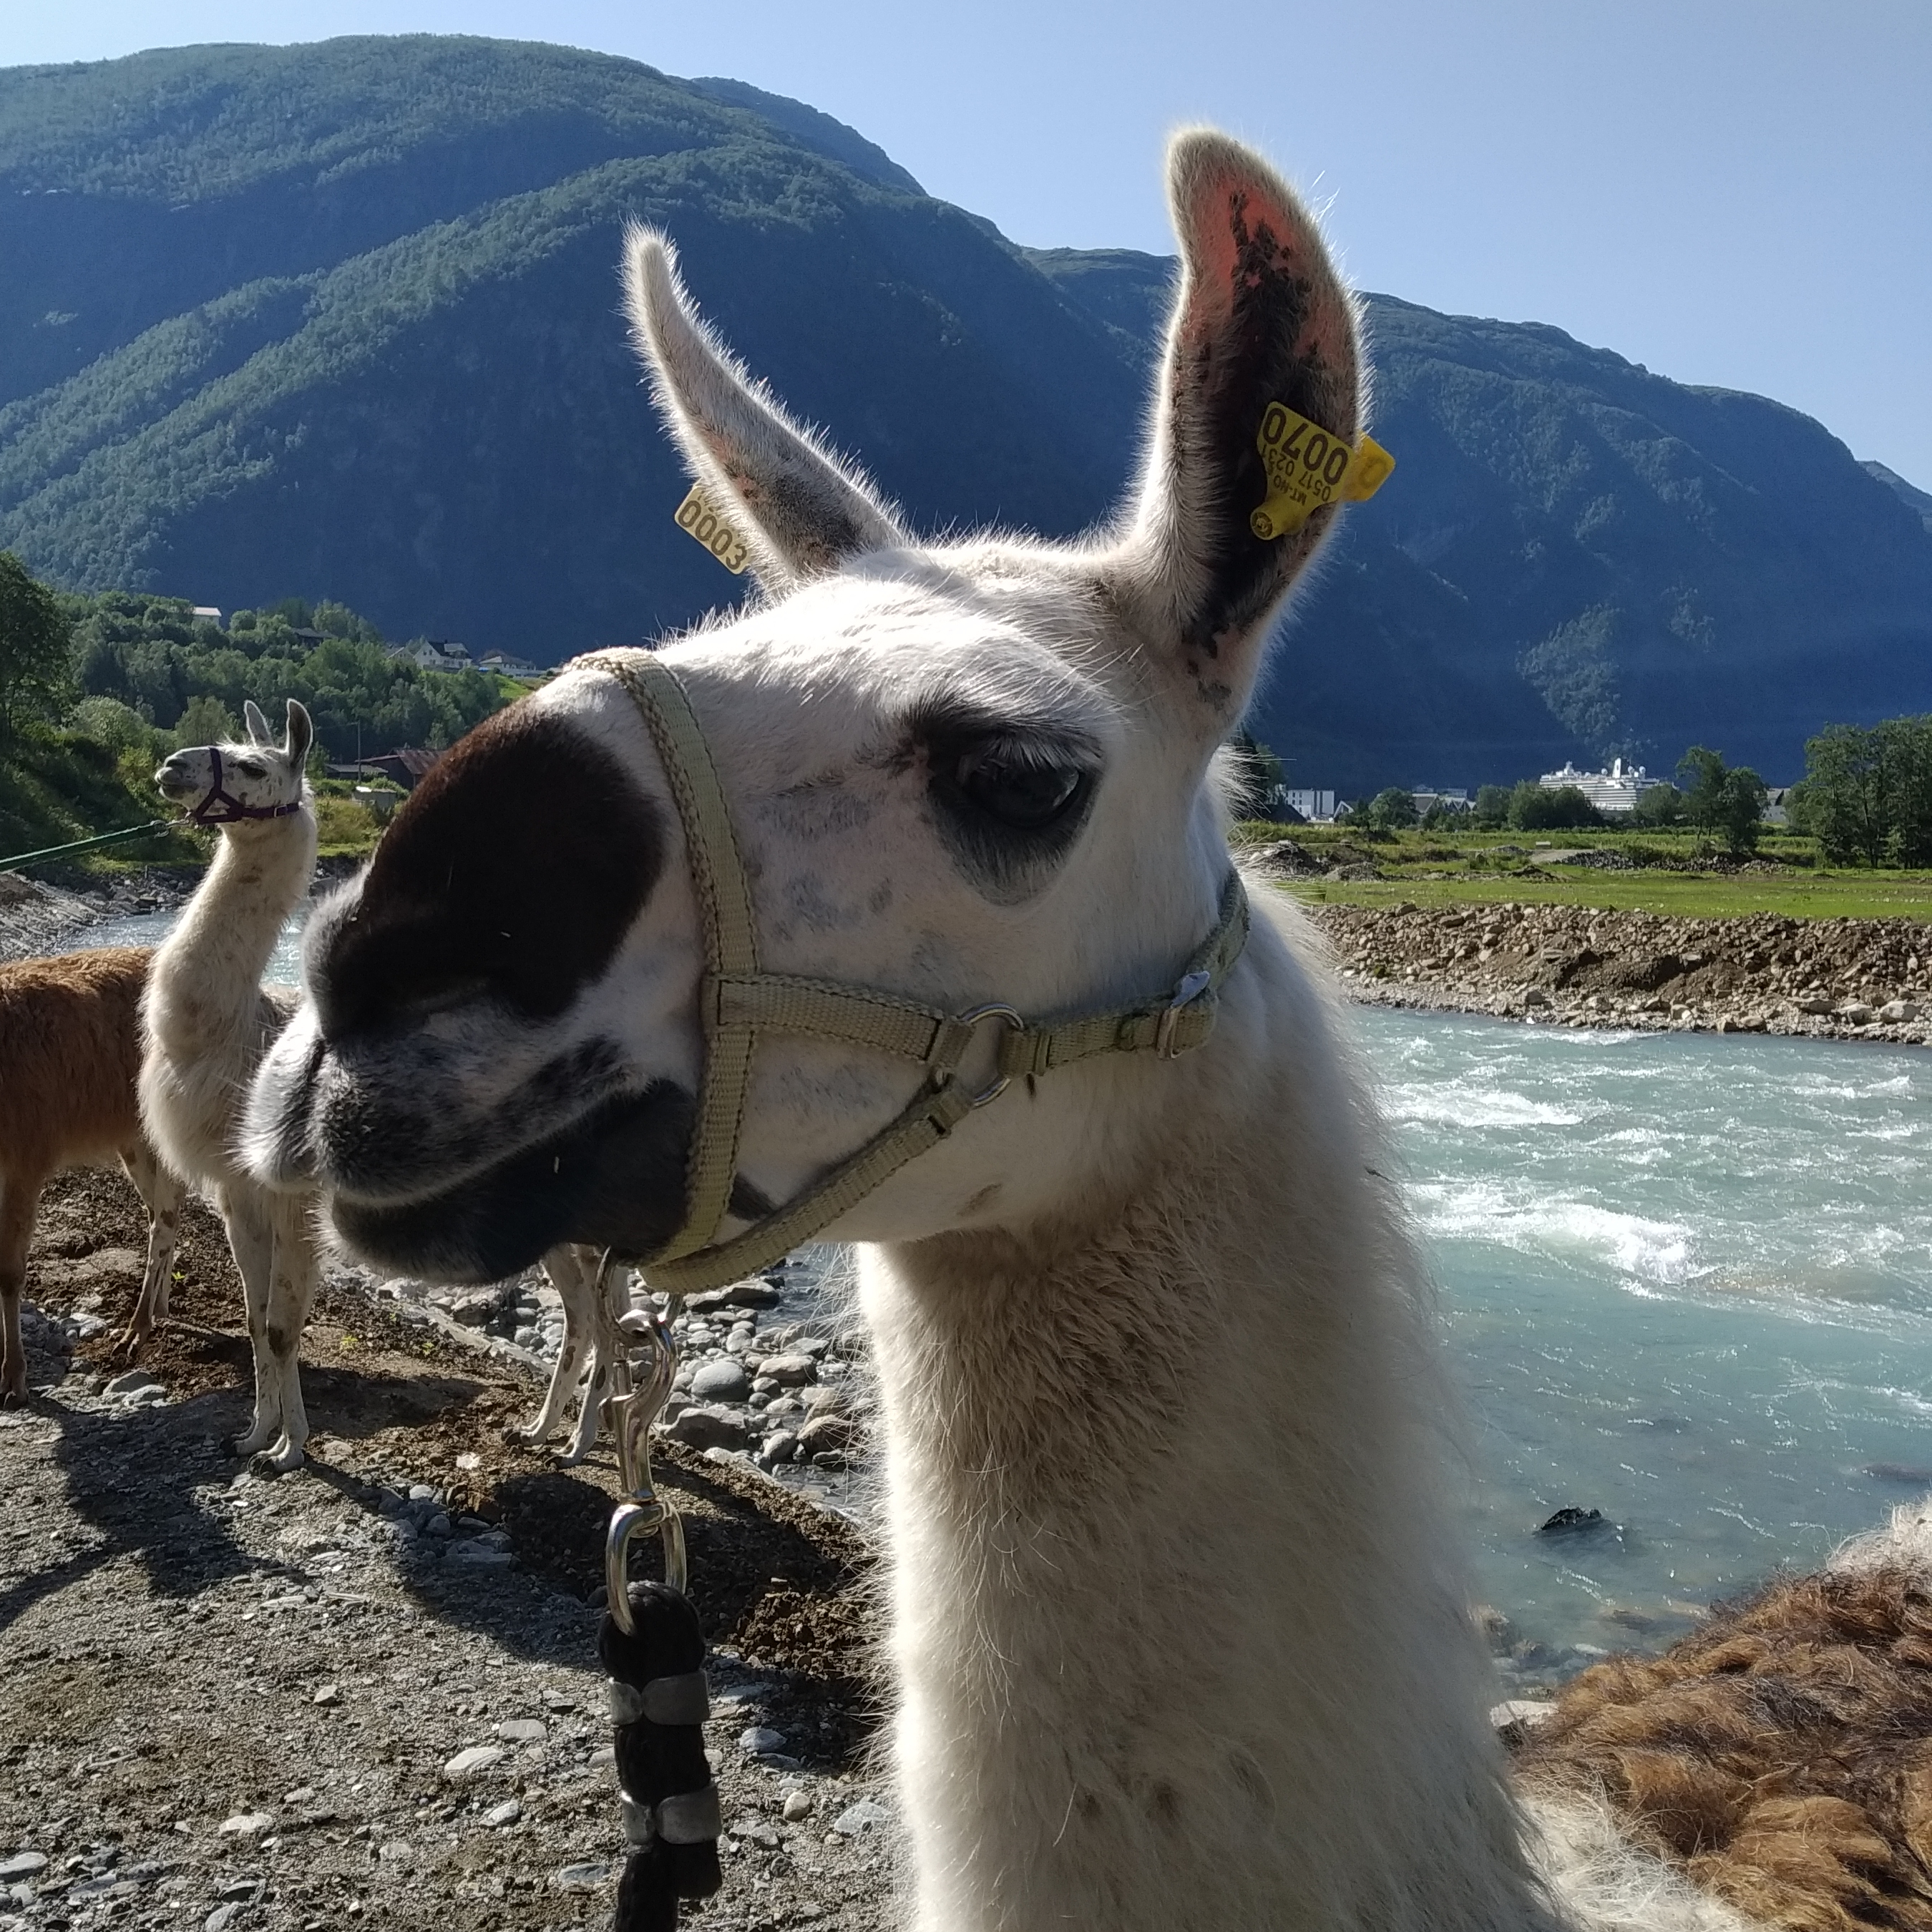
\includegraphics[width=0.25\textwidth]{img/personal_images/llama.jpg}
    }
    \subfloat[\textit{Meerkat} (299)]{
        \label{ref_pi12}
        \includegraphics[width=0.25\textwidth]{img/personal_images/meerkat.jpg}
    }
    \newline
    % images 13-16
    \subfloat[\textit{English springer} \newline \centerline{(217)}]{
        \label{ref_pi13}
        \includegraphics[width=0.25\textwidth]{img/personal_images/megan.jpg}
    }
    \subfloat[\textit{Running shoe} (770)]{
        \label{ref_pi14}
        \includegraphics[width=0.25\textwidth]{img/personal_images/running_shoes.jpg}
    }
    \subfloat[\textit{Tabby} (281)]{
        \label{ref_pi15}
        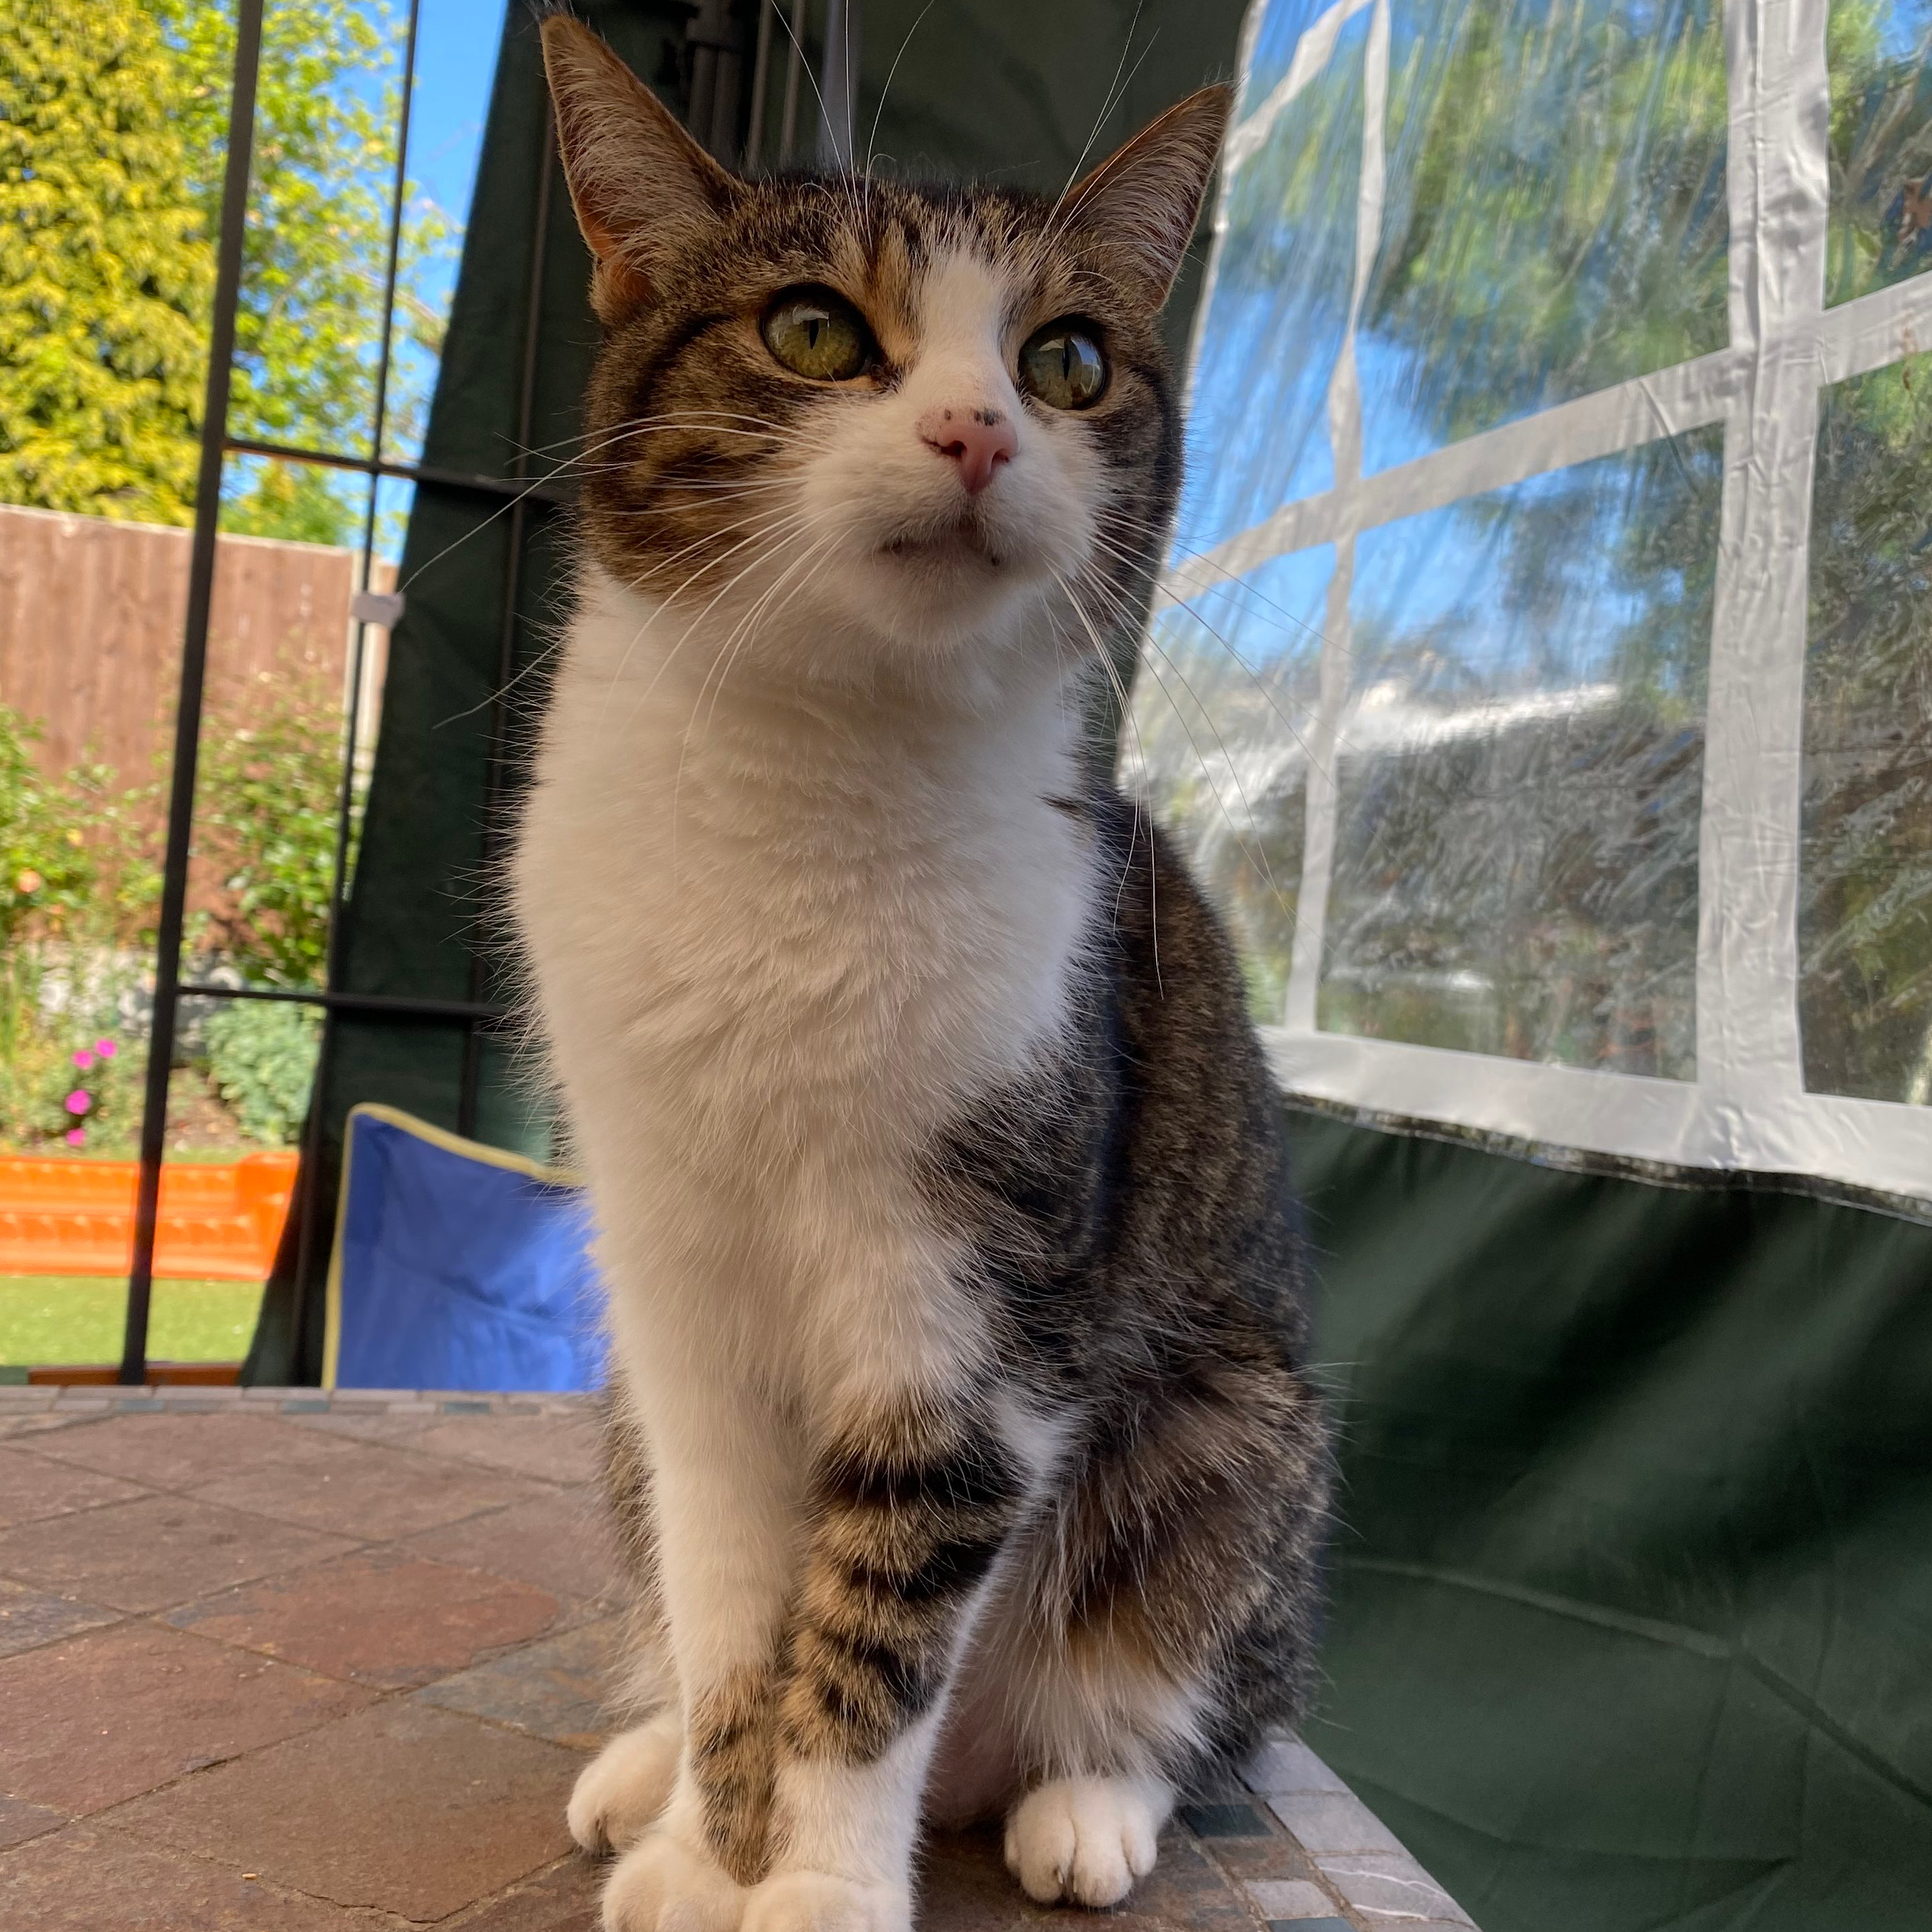
\includegraphics[width=0.25\textwidth]{img/personal_images/tabby.jpg}
    }
    \subfloat[\textit{Wardrobe} (894)]{
        \label{ref_pi16}
        \includegraphics[width=0.25\textwidth]{img/personal_images/wardrobe.jpg}
    }
    
    \caption{Slike korištene za generiranje suparničkih primjera te njihove ispravne labele}
    \label{ref_personal_image_table}
\end{figure}

\section{Izlazi modela na nepromijenjenim slikama iz osobnog skupa}



\begin{sazetak}
Današnji konvolucijski modeli postižu visoku točnost u području raspoznavanja objekata. Način rada dubokih modela je još uvijek vrlo teško ili nemoguće interpretirati, a dodatan razlog za brigu predstavljaju i nedavno otkriveni neprijateljski primjeri. Neprijateljski primjeri su slike s dodatnim teško uočljivim perturbacijama koje potiču model na pogrešnu klasifikaciju. Pokazalo se da je vrlo lagano konstruirati brze i efikasne napade na postojeće modele, međutim  ubrzo su se pojavile i obrane protiv takvih napada. Ti početni napadi su se oslanjali na pristup mreži i poznavanju arhitekture, a obrane od takvih napada se temelje na "prikrivanju" potrebnih informacija, kao što su gradijenti.

\kljucnerijeci{duboko učenje, klasifikacija, konvolucijske neuronske mreže, računalni vid, suparnički primjeri, neprijateljski primjeri, obrana.}
\end{sazetak}

\engtitle{Defending Deep Convolutional Models from Adversarial Examples}
\begin{abstract}
Deep neural networks can achieve very high accuracy in many applications such as image classification. However, most of these deep models are difficult to interpret and they are often sensitive to the so-called adversarial examples. This feature opens up the possibility of maliciously designing adversarial examples that could deceive a deep learning system. 

\keywords{deep learning, classification, convolutional neural networks, computer vision, adversarial attacks, defense.}
\end{abstract}
\end{document}
